\chapter{Introdução}

Imagens e vídeos de forma geral podem conter uma quantidade significativa de informações valiosas, que com a ajuda da tecnologia, há possibilidade de serem extraídas em forma de texto de maneira automática. Essas informações registradas e processadas têm utilidade para os mais variados objetivos, como pesquisa, consultas ou até mesmo questões mais específicas. Entretanto, para que isso aconteça, é necessária uma série de técnicas como por exemplo detecção, localização, aprimoramento, extração e reconhecimento de texto \cite{jung2004text}.

Existe uma gama de aplicações que utilizam essas técnicas citadas, fazendo uso de bibliotecas de visão computacional para linguagens de programação. Algumas dessas aplicações são bem conhecidas, como a biometria por impressões digitais ou pela íris do olho humano, e o reconhecimento facial, encontrado em muitas redes sociais atuais \cite{caap}. Existem também certas soluções para reconhecimento ótico de caracteres, geralmente utilizados em \textit{scanners}. Essas soluções são conhecidas como OCRs (\textit{Optical Character Recognition}) sendo também parte do conceito de visão computacional. 

Diversas bibliotecas OCRs estão disponíveis para uso, como por exemplo a Tesseract-OCR \cite{tesseract-ocr}, a GOCR \cite{GOCR}, a OCRAD \cite{OCRAD} e outras. Todas são bibliotecas de reconhecimento de texto com licença gratuita. A Tesseract, GOCR e OCRAD compõe grande parte deste trabalho. 

O problema é que não existem meios de um sistema de computador interpretar uma imagem da mesma forma que um ser humano \cite{rudek}. Por esse motivo, tem-se a necessidade do uso de técnicas, pois a função básica realizada por um computador é a execução de programas, que consiste em um conjunto de instruções armazenadas na memória \cite{stallings}, e a visão computacional procura integrar as áreas de processamento digital de imagens e inteligência artificial, tendo como objetivo a obtenção de algoritmos capazes de interpretar o conteúdo visual das imagens \cite{avancosvisao}. Um exemplo seria a leitura de placas de veículos, pois facilmente um ser humano consegue identificar as letras e números contidos na placa, entretanto um computador sem um algoritmo especializado não.

Existem alguns softwares e projetos que buscam fazer o reconhecimento de placas automotivas como \cite{openalpr}, \cite{licenseplaterecognition}, \cite{GOCR}, \cite{chang2004automatic}, \cite{hegt1998high}, \cite{nijhuis1995car}. Um dos que mais são conhecidos chama-se OpenALPR, que traz bons resultados de precisão, e também é capaz de encontrar uma placa em meio a um cenário, para então extrair as informações. Este software, que ainda está em desenvolvimento, possui uma comunidade ampla de desenvolvedores, não contendo ainda uma documentação formal disponível ao público. Há uma versão do projeto do software com licença AGPL e também versões comerciais, contudo ele reconhece apenas placas norte americanas e europeias \cite{openalpr}.

Este trabalho resume-se em reconhecer caracteres de imagens de placas de licenciamento de veículos brasileiros, transformando-os em texto simples. Assim podem ser aplicadas ações sobre este texto como consultas na base fiscal do Denatran. No âmbito de reconhecimento de placas brasileiras, \citeonline{licenseplaterecognition} apresenta uma solução que possui seis processos, observados na \autoref{fig:diagramasistema}, são esses:

\begin{alineas}
\item Captura: Submete a imagem que será a entrada do sistema. A imagem pode ser obtida através de uma câmera \textit{webcan} ou qualquer dispositivo semelhante. 
\item Pré-processamento: Trata a imagem para que as condições da localização da placa aumentem.
\item Localização: Identifica as bordas na imagem.
\item Validação: Encontra por definitivo a placa.
\item Segmentação: Corta a imagem da placa encontrada no processo anterior.
\item Leitura OCR: Trata a imagem recebida da etapa de segmentação. Passar por um leitor OCR identificando os caracteres contidos e retornando em forma de texto simples. 
\end{alineas}

\begin{figure}[htbp]
\caption{\label{fig:diagramasistema}Diagrama de sistema de detecção de placa automotiva}
\begin{center}
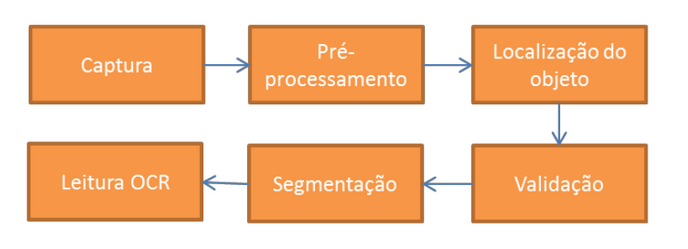
\includegraphics[width=.9\textwidth]{figuras/f1c1.png}
\end{center}
\legend{Fonte: \citeonline{licenseplaterecognition}}
\end{figure}


O autor fez uso da biblioteca Tesseract-OCR \cite{tesseract-ocr}, mostrando um desempenho consideravelmente bom, dependendo das circunstâncias em que se encontram as etapas de validação e segmentação. Porém, foram necessários treinamentos do Tesseract-OCR, que foram considerados ``trabalhosos'' pelo autor. Certos testes resultaram em falhas, devido a alguns problemas que serão citados ao longo do trabalho. 

Este trabalho então, tem como proposta principal implementar uma solução semelhante com o uso das bibliotecas de OCR "GOCR" e "OCRAD", testando dessa forma se é possível manter o desempenho em relação a biblioteca Tessaract-OCR sem a utilização de treinamentos. Vale enfatizar que o fato de utilizar diferentes OCRs afeta diretamente no resultado, podendo ser melhor ou não.

O restante desse trabalho está dividido em cinco capítulos. O capítulo 2 trata a respeito do que é visão computacional e OCR, explicando conceitos de forma geral e apresentando certas aplicações que o utilizam. O capítulo 3 explora a ferramenta OpenCV e suas funcionalidades dando ênfase nas que serão utilizadas para a solução, também serão vistas algumas questões sobre o GOCR o OCRAD e o Tesseract, e para conclusão do capítulo serão abordados conceitos básicos de processamento de imagens. O Capítulo 4 aborda o desenvolvimento. O capítulo 5 trata-se da conclusão.
